\subsection{Trajectoires}

On rappelle que dans un réferentiel \((Rg)\) galliléen, pour une force centrale newtonienne, on a : 
\[
    m\vv{a} = F(r) \vv{u}_{r}, F(r) = \frac{k}{r^{2}}
\] 
D'où par projection sur \(\vv{u}_{r}\), on a : 
\[
    -l^{2}u^{2} \left[ \frac{d^{2}u}{d \theta^{2}} +u  \right]m = ku^{2}
\] 

\begin{align*}
    -l^{2}u^{2} \left[ \frac{d^{2}u}{d \theta^{2}} +u  \right]m &= ku^{2} \\
    \implies \frac{d^{2}u}{d \theta^{2}} +u &= -\frac{k}{ml^{2}} 
\end{align*}

On résoud l'équation différentielle : 
\begin{align*}
    \intertext{Solution homogène : }
    \frac{d^{2}u_{h}}{d \theta^{2}} + u_{h} &= 0 \\
    \implies u_{h} &= A \cos \left( \theta(t) -\theta_{\text{0}} \right) 
    \intertext{Solution particulière : \(\frac{d^{2}u_{h}}{d \theta^{2}} = 0\) }   
    \implies u_{p} &= -\frac{k}{ml^{2}}\\
    \intertext{Solution générale} : 
    u(\theta) &= u_{h} + u_{p} = A\cos\left( \theta -\theta_{\text{0}} \right) - \frac{k}{ml^{2}} 
\end{align*}
Or \(r = \frac{1}{u}\), d'où :
\[
    \boxed{r(\theta) = \frac{-\frac{ml^{2}}{k}}{1-\frac{Aml^{2}}{k}\cos\left( \theta - \theta_{\text{0}} \right)}}
\] 

Or la formule générale d'un conique en coordonnées polaires est : 
\[
    r = \frac{p}{1+e\cos(\theta-\theta_{\text{0}})} 
\]
\begin{enumerate}
    \item Si \(e = 0\), la trajectoire est circulaire
    \item Si \(e \in \left[ 0;1 \right]\), la trajectoire est une  ellipse. 
    \item Si \(e =1\), la trajectoire est une parabole de foyer \(O\)
    \item Si \(e >1\) la trajectoire est hyperbolique
\end{enumerate}

\begin{figure}[!htb]
    \centering
    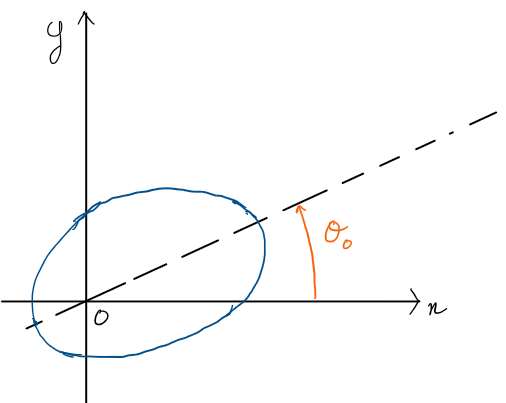
\includegraphics[width=0.4 \textwidth]{SCHEMA3-6.png}
    \caption{Représentation d'une trajectoire elliptique. On peut toujours prendre \(\theta_{0} = 0\) }
    \label{fig:SCHEMA3-6}
\end{figure}

\begin{figure}[!htb]
    \centering
    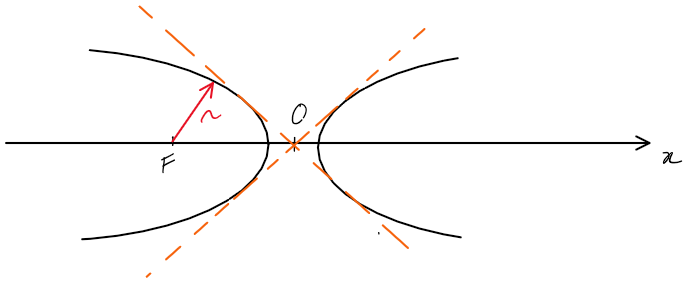
\includegraphics[width=0.6 \textwidth]{SCHEMA3-7.png}
    \caption{Représentation d'une trajectoire hyperbolique}
    \label{fig:SCHEMA3-7}
\end{figure}



\begin{definition}[Axes d'une ellipse]
    On appelle \(a = OA\) le demi grand axe de l'ellipse, \(b =OB\) le demi petit axe de l'ellipse. Les deux sont liés par la formule : \(p = \frac{b^{2}}{a}\).  
\end{definition}

\begin{figure}[!htb]
    \centering
    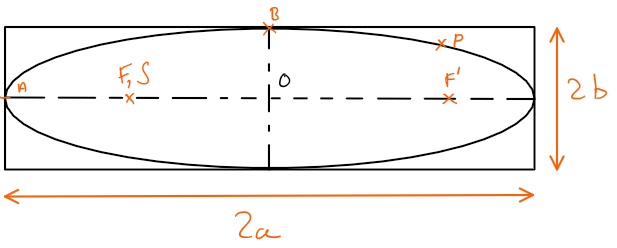
\includegraphics[width=0.8 \textwidth]{SCHEMA3-8.png}
    \caption{Caractéristiques d'une ellipse}
    \label{fig:SCHEMA3-8}
\end{figure}


\[
    r = \frac{p}{1+e\cos \theta}
\]

\begin{corollary}[Distances maximales et minimales]
    On a donc : 
    \begin{enumerate}
        \item La distance maximale, appelée apoastre (aphélie autour du soleil) : \(r_{\max } = \frac{p}{1-e}\)
        \item La distance minimale, appelée périastre (périhélie autour du soleil) : \(r_{\min} = \frac{p}{1+e}\) 
    \end{enumerate}
\end{corollary}

\subsection{Vitesse aérolaire, troisième loi de Kepler}

\begin{theorem}[Troisième loi de Kepler]
    Pour un objet en orbite elliptique autour d'un astre de période \(T\) et de demi grand axe \(a\), on a : 
    \[
        \frac{T^{2}}{a^{3}} = \frac{4\pi^{2}}{GM}
    \]
\end{theorem}
\newpage
\begin{explanation}
    On rappelle que la vitesse aérolaire \(\frac{d \mathcal{A}}{dt} = \frac{l}{2}\) est constante et que l'aire d'une ellipse est \(\pi ab\).
    \begin{align*}
        \frac{\Delta \mathcal{A}}{\Delta t} &= \frac{l}{2} \\
        \implies \frac{\pi ab}{T} &= \frac{l}{2} \\
        \implies \frac{\pi^{2}a^{2}b^{2}}{T^{2}} &= \frac{l^{4}}{4}\\
        \intertext{Or \(p = \frac{b^{2}}{a} = -\frac{ml^{2}}{k} = \frac{l^{2}}{GM}\) }
        \implies c^{2} &= \frac{GMb^{2}}{a}\\
        \implies \frac{\pi^{2}a^{2}b^{2}}{T^{2}} &= \frac{GMb^{2}}{4a}\\
        \implies \frac{a^{3}}{T^{2}} = \frac{GM}{4\pi^{2}} \,\square 
    \end{align*}
\end{explanation}